\documentclass{hitec}
\usepackage{graphicx}
\usepackage{lscape}
\usepackage{longtable}
\usepackage{subcaption} 
\usepackage[space]{grffile}
\usepackage{pdfpages}
\usepackage{listings}
\usepackage{amsmath}
\definecolor{mygray}{rgb}{0.5,0.5,0.5}
\lstset{  breaklines=true, numbers=left, numberstyle=\tiny\color{mygray}, keepspaces=true }

\usepackage{siunitx} %https://tex.stackexchange.com/questions/413312/how-to-put-angstrom/413317

\usepackage{titlesec}
\usepackage{hyperref}
\usepackage{enumitem} %https://www.latex-tutorial.com/tutorials/lists/

%\usepackage{wasysym}
\usepackage{mathabx}

% https://shantoroy.com/latex/add-subfig-in-latex/
\usepackage{caption}
\usepackage{subcaption}

\usepackage{pgfplots} % https://www.tug.org/TUGboat/tb31-1/tb97wright-pgfplots.pdf

\usepackage{listings} % https://en.wikibooks.org/wiki/LaTeX/Source_Code_Listings

\usepackage{natbib}

\usepackage{xcolor}
\hypersetup{
	colorlinks,
	linkcolor={blue!50!black},
	citecolor={blue!50!black},
	urlcolor={blue!80!black}
}

\titleclass{\subsubsubsection}{straight}[\subsection]

\newcounter{subsubsubsection}[subsubsection]
\renewcommand\thesubsubsubsection{\thesubsubsection.\arabic{subsubsubsection}}
\renewcommand\theparagraph{\thesubsubsubsection.\arabic{paragraph}} % optional; useful if paragraphs are to be numbered

\titleformat{\subsubsubsection}
{\normalfont\normalsize\bfseries}{\thesubsubsubsection}{1em}{}
\titlespacing*{\subsubsubsection}
{0pt}{3.25ex plus 1ex minus .2ex}{1.5ex plus .2ex}

\makeatletter
\renewcommand\paragraph{\@startsection{paragraph}{5}{\z@}%
	{3.25ex \@plus1ex \@minus.2ex}%
	{-1em}%
	{\normalfont\normalsize\bfseries}}
\renewcommand\subparagraph{\@startsection{subparagraph}{6}{\parindent}%
	{3.25ex \@plus1ex \@minus .2ex}%
	{-1em}%
	{\normalfont\normalsize\bfseries}}
\def\toclevel@subsubsubsection{4}
\def\toclevel@paragraph{5}
\def\toclevel@paragraph{6}
\def\l@subsubsubsection{\@dottedtocline{4}{7em}{4em}}
\def\l@paragraph{\@dottedtocline{5}{10em}{5em}}
\def\l@subparagraph{\@dottedtocline{6}{14em}{6em}}
\makeatother

\setcounter{secnumdepth}{4}
\setcounter{tocdepth}{4}


\title{Radiation Dose in Composites}
\author{Anthony M. DeStefano}
\company{NASA, MSFC, EV44}
\confidential{\textbf{-- For internal NASA and partners use only --}}
\usepackage{hyperref} 
\begin{document}
\maketitle
\pagenumbering{roman}

\tableofcontents
\listoffigures
\listoftables
\newpage



%\section*{Contributing Author List}
%\addcontentsline{toc}{section}{Contributing Author List}



\cleardoublepage
\pagenumbering{arabic}
%%%%%%%%%%%%%%%%%%%%%%%%%%%%%%%%%%%%%%%%%%%%%%%%%%%%%%%%%%%%%%%%%%
%%%%%%%%%%%%%%%%%%%%%%%%%%%%%%%%%%%%%%%%%%%%%%%%%%%%%%%%%%%%%%%%%%
%\section{Executive Summary}
%
%
%
%\newpage
%%%%%%%%%%%%%%%%%%%%%%%%%%%%%%%%%%%%%%%%%%%%%%%%%%%%%%%%%%%%%%%%%%
%%%%%%%%%%%%%%%%%%%%%%%%%%%%%%%%%%%%%%%%%%%%%%%%%%%%%%%%%%%%%%%%%%
\section{Executive Summary}

%%%%%%%%%%%%%%%%%%%%%%%%%%%%%%%%%%%%%%%%%%%%%%%%%%%%%%%%%%%%%%%%%%
%%%%%%%%%%%%%%%%%%%%%%%%%%%%%%%%%%%%%%%%%%%%%%%%%%%%%%%%%%%%%%%%%%
\section{Introduction}

%%%%%%%%%%%%%%%%%%%%%%%%%%%%%%%%%%%%%%%%%%%%%%%%%%%%%%%%%%%%%%%%%%
%%%%%%%%%%%%%%%%%%%%%%%%%%%%%%%%%%%%%%%%%%%%%%%%%%%%%%%%%%%%%%%%%%
\section{Material Properties}

Basic material properties that are essential in the estimation of dose are material density and thickness. For higher fidelity calculations of dose, the material stoichiometry is required. If a particular material is layered, the material properties of each layer would be needed. Each layer would assumed to be homogeneous in a particular elemental composition.

In Sections \ref{ssec:composites} and \ref{ssec:MLI}, we discuss assumptions in material properties of composites and multi-layered insulation.

%%%%%%%%%%%%%%%%%%%%%%%%%%%%%%%%%%%%%%%%%%%%%%%%%%%%%%%%%%%%%%%%%%
%%%%%%%%%%%%%%%%%%%%%%%%%%%%%%%%%%%%%%%%%%%%%%%%%%%%%%%%%%%%%%%%%%
\subsection{Composites}\label{ssec:composites}

To first order, composites are typically composed of a fiber material and a matrix that is dominated by a resin bonding material with additives as a minor component.

\subsubsection{Density}
In this analysis, three fiber materials were considered:


\begin{table}[h]\centering
	\caption{List of approximate fiber densities.}\label{tab:fiber_dens}
	\begin{tabular}{|c | c |}\hline
		Fiber Type & Density [g cm$^{-3}$] \\\hline
		Glass	& 1.9 \\\hline
		Aramid	& 1.4 \\\hline
		Carbon	& 1.6 \\\hline	
	\end{tabular}
\end{table}

In composites of interest, the mass percentage of resin is approximately $33-35\%$ (e.g., for composite overwrapped pressure vessels (COPVs)). An example density for epoxy resin is about $1.3$ g cm$^{-3}$ \citep{joven2013characterization}. Therefore, we can approximate the three composite materials as:

\begin{table}[h]\centering
	\caption{List of approximate composite densities using fiber densities from Table \ref{tab:fiber_dens}, an epoxy resin density of $1.3$ g cm$^{-3}$, and an epoxy resin mass percentage of $33-35\%$.}\label{tab:comp_dens}
	\begin{tabular}{|c | c |}\hline
		Composite Type & Density [g cm$^{-3}$] \\\hline
		Glass + epoxy	& 1.70 \\\hline
		Aramid + epoxy	& 1.37 \\\hline
		Carbon + epoxy	& 1.50 \\\hline	
	\end{tabular}
\end{table}

\subsubsection{Thickness}
For a given environment, radiation damage to composites is widely dependent on composition, manufacturing processes, size/thickness, and if any shielding is present. In this analysis, a range of thicknesses are considered based on the following components:

\begin{table}[h]\centering
	\caption{List of representative materials made of composites with a range of thicknesses.}\label{tab:thickness_comp}
	\begin{tabular}{|c | c | c |}\hline
		Composite Component & Min Thickness [mm] & Max Thickness [mm] \\\hline
		COPV & 1.5 & 19 \\\hline
		Landing struts	& 1.5 & 19 \\\hline
		Sandwich panels/Face sheets	& 0.8 & 6.5 \\\hline
		Solid laminate	& 1 & 19 \\\hline	
	\end{tabular}
\end{table}

\subsubsection{Stoichiometry}

At the time of writing, no representative material stoichiometric information has been given. Therefore, placeholder values are assumed that are used in this analysis.

In the SRIM software package, there is a list of common compounds, one of which is epoxy. For the three fiber types shown in Table \ref{tab:fiber_dens}, we assume the most basic elemental composition. Stoichiometry for the epoxy and the fiber materials are shown in Table \ref{tab:stoichiometry}.

\begin{table}[h]\centering
	\caption{The epoxy resin composition is taken from the common compound table in SRIM. Glass fiber is assumed to be strictly made of silicon-based glass. The aramid fiber is assumed to be a Nomex or Kevlar type aramid. Carbon fiber is assumed to be made of only carbon.}\label{tab:stoichiometry}
	\begin{tabular}{|c | c |}\hline
		Material & Stoichiometry [element-count] \\\hline
		Epoxy resin & H-19, C-18, O-3 \\\hline
		Glass fiber & O-2, Si-1 \\\hline
		Aramid fiber & H-2, C-14, N-2, O-2  \\\hline
		Carbon fiber & C-1  \\\hline	
	\end{tabular}
\end{table}

If a homogenized substance composed of the epoxy and fiber material is assumed, a net stoichiometry list (see Table \ref{tab:stoichiometry-net}) can be built using the assumption that the epoxy is $33-35\%$ of the total weight of the composite. Densities from Table \ref{tab:comp_dens} should be used for each of the composites.

\begin{table}[h]\centering
	\caption{Stoichiometry for each composite is given where the epoxy weight is $33-35\%$ of the total mass.}\label{tab:stoichiometry-net}
	\begin{tabular}{|c | c |}\hline
		Material & Stoichiometry [element-count] \\\hline
		Glass composite & H-19, C-18, O-21, Si-9 \\\hline
		Aramid composite & H-23, C-46, N-4, O-7  \\\hline
		Carbon composite & H-19, C-62, O-3  \\\hline	
	\end{tabular}
\end{table}

\subsubsection{Proton Stopping Distance}
\label{sssec:ProtonStoppingDistance}

The effective stopping (shielding) capabilities for a given proton energy of a composite material can be estimated using SRIM. Using the ion stopping and range table calculator in SRIM, we plug in the stoichiometry (Table \ref{tab:stoichiometry-net}) and density (Table \ref{tab:comp_dens}) for each composite material. The generated output provides the projected range, longitudinal and lateral straggling as a function of ion energy. To estimate the maximum stopping distance of the proton, we take the projected range and add half of the lateral straggling, since we are assuming a normally incident beam. The proton energy range used to generate the stopping distance tables is $10$ keV to $1$ GeV, completely encompassing the typical energy range of solar energetic particles (SEPs). See Listings~\ref{lst:glass_composite}-\ref{lst:aluminum} in Appendix \ref{asec:IonStoppingRangeTables} for the stopping distance tables.

The maximum stopping distance as a function of ion energy can be fit by a double power law given by
\begin{equation}\label{eq:energy_vs_stopping_distance}
E[keV] = \frac{a}{\left(\frac{x[mm]}{c}\right)^{-b} + x[mm]^{-d}},
\end{equation}
where the ion energy $E$ is in keV and the maximum stopping distance $x$ is in mm. The constant $a$ can be thought of as the largest ion energy (in keV) that roughly $1$ mm of material can stop completely. The constant $c$ defines the length scale (in mm) at which low energy ions are affected. The index $b$ is the power law relation that dominates for thin materials (i.e., on the order of $c$ and smaller) and the index $d$ is the power law relation that dominates for thick materials (i.e., much greater than $c$).

For a given material, keeping the stoichiometry the same, changing the density only changes the constants $a$ and $c$. If the initial density is $\rho_0$ and the new density is $\rho_1$, where $\alpha = \rho_1/\rho_0$, the ion energy is then given by
\begin{equation}\label{eq:energy_vs_stopping_distance_rescaled}
E[keV] = \frac{a\alpha^d}{\left(\frac{x[mm]}{c\alpha^{\frac{d}{b}-1}}\right)^{-b} + x[mm]^{-d}},
\end{equation}
where new constants $a'$ and $c'$ can be defined as
\begin{align}
a' &= a\alpha^d, \\
c' &= c\alpha^{\frac{d}{b}-1},
\end{align}

Fitting Listings~\ref{lst:glass_composite}-\ref{lst:aluminum} with Equation \ref{eq:energy_vs_stopping_distance}, the parameters $a$, $b$, $c$, and $d$ are given in Table~\ref{tab:stopping_distance}.

\begin{table}[h]\centering
	\caption{Parameters to the double power law fit of the proton energy as a function of maximum stopping distance of composites compared to aluminum of density $2.702$ g cm$^{-3}$.}\label{tab:stopping_distance}
	\begin{tabular}{|c | c | c | c | c |}\hline
		Material & a [keV] & b & c [mm] & d \\\hline
		Glass composite  & 1.068E4 & 1.668 & 1.31E-2 & 0.5759 \\\hline
		Aramid composite & 9.89E3  & 1.706 & 1.23E-2 & 0.5721  \\\hline
		Carbon composite & 1.039E4 & 1.699 & 1.16E-2 & 0.5717 \\\hline
		Aluminum         & 1.270E4 & 1.529 & 1.49E-2 & 0.5794 \\\hline
	\end{tabular}
\end{table}

In order to compare the stopping distance of equal density materials, we rescale the composites to that of aluminum at $2.702$ g cm$^{-3}$ using Equation \ref{eq:energy_vs_stopping_distance_rescaled}. The rescaled parameters are given in Table \ref{tab:stopping_distance_rescaled}.

\begin{table}[h]\centering
	\caption{Parameters to the double power law fit of the proton energy as a function of maximum stopping distance of composites rescaled to the density of aluminum compared to aluminum of density $2.702$ g cm$^{-3}$.}\label{tab:stopping_distance_rescaled}
	\begin{tabular}{|c | c | c | c | c |}\hline
		Material & a [keV] & b & c [mm] & d \\\hline
		Glass composite  & 1.395E4 & 1.668 & 9.67E-3 & 0.5759 \\\hline
		Aramid composite & 1.46E4  & 1.706 & 7.83E-3 & 0.5721  \\\hline
		Carbon composite & 1.455E4 & 1.699 & 7.85E-3 & 0.5717 \\\hline
		Aluminum         & 1.270E4 & 1.529 & 1.49E-2 & 0.5794 \\\hline
	\end{tabular}
\end{table}

Examining Table \ref{tab:stopping_distance_rescaled}, for the list of composites in this analysis, the large thickness range (i.e., much greater than $c$) is independent of material type and density. The small-scale range $c$ for the composites is on the order of $8-10$ $\mu$m and smaller, whereas the small-scale range for aluminum is roughly $15$ $\mu$m and smaller. The index parameter for small scales $b$ seems to be strongly material dependent, which in turn implies the maximum stopped energy to be strongly dependent on materials for thin materials. Observing the $a$ parameter, the composites tend to have greater stopping capability of protons compared to aluminum. This may have to do with the large number of hydrogen atoms present in the composites themselves, since the collision cross section between hydrogen atoms and protons is higher than large-Z materials.

For larger thicknesses $x \gg c$ (i.e., thicknesses greater than roughly 0.5 mils), we can approximate Equation \ref{eq:energy_vs_stopping_distance} as
\begin{equation}\label{eq:energy_vs_stopping_distance-large_dist}
E[keV] \sim a x[mm]^d.
\end{equation}
In order to use the material density to scale the equivalent thickness, a correction factor is needed if data on aluminum is used to estimate stopping power of composites. These scale factors $\kappa$ can be computed as
\begin{equation}
\kappa_{\text{composite}} = \left(\frac{a_{\text{composite}}}{a_{\text{Al}}}\right)^{1/d}.
\end{equation} 

Therefore, when rescaling the composites to aluminum equivalent thicknesses, the true scaling is given by (taking $d\approx 0.575$)
\begin{equation}\label{eq:al_equiv_thickness_conversion}
x_{\text{Al equiv}} = \kappa_{\text{composite}}\frac{\rho_{\text{composite}}}{\rho_{\text{Al}}}x_{\text{composite}},
\end{equation}
where $x_{\text{composite}}$ is the composite thickness and $x_{\text{Al equiv}}$ is the corrected aluminum equivalent thickness. The correction factors for the composites studied in this analysis are given in Table \ref{tab:correction_factors}.

\begin{table}[h]\centering
	\caption{Length scale correction factors to aluminum equivalent modeling of composites.}\label{tab:correction_factors}
	\begin{tabular}{|c | c |}\hline
		Material & $\kappa_{\text{composite}}$ \\\hline
		Glass composite  & 1.177 \\\hline
		Aramid composite & 1.272   \\\hline
		Carbon composite & 1.266 \\\hline
	\end{tabular}
\end{table}

With the correction factors greater than one, an interpretation can be that for a composite and aluminum coupon of similar areal density, more energy will be absorbed (i.e., more ionizing dose) by the composite per areal density since higher energy protons can be stopped in the composite compared to the aluminum equivalent (i.e., the $a$ parameters for the composites are greater than that for aluminum in Table~\ref{tab:stopping_distance_rescaled}). For example, in order to have the same limiting energy as glass composite, the aluminum equivalent thickness must be increased by $17.7\%$, according to Table \ref{tab:correction_factors}.

%%%%%%%%%%%%%%%%%%%%%%%%%%%%%%%%%%%%%%%%%%%%%%%%%%%%%%%%%%%%%%%%%%
%%%%%%%%%%%%%%%%%%%%%%%%%%%%%%%%%%%%%%%%%%%%%%%%%%%%%%%%%%%%%%%%%%
\subsection{Multi-layered Insulation (MLI)}\label{ssec:MLI}

Multi-layered insulation, or MLI, is used on spacecraft to aid in thermal management and certain types of radiation and contamination protection. In Chapter 5 of the Spacecraft Thermal Control Handbook \citep{donabedian2003spacecraft}, details about MLI applications are descried. Table \ref{tab:MLI} lists separate components of MLI taken from \cite{donabedian2003spacecraft}.

\begin{table}[h]\centering
	\caption{Various components and layers of MLI and their average densities and thicknesses.}\label{tab:MLI}
	\begin{tabular}{|c | c | c | c |}\hline
		Name & Layer & Density [g cm$^{-3}$] & Thickness [mils] \\\hline
		Beta cloth            & outer     & 1.185 & 8 \\\hline
		Aluminized beta cloth & outer     & 1.355 & 8 \\\hline
		Kapton                & outer     & 1.50  & 0.5 - 5 \\\hline
		Teflon                & outer     & 2.17  & 0.5 - 5 \\\hline
		Aluminized Kapton     & interior  & 1.50  & 0.3 - 5 \\\hline
		Goldized Kapton       & interior  & 1.50  & 0.3 - 5 \\\hline
		Aluminized mylar      & interior  & 1.38  & 0.25 - 5 \\\hline
		Dacron netting        & separator & 0.04  & 6.5 \\\hline
		Nomex netting         & separator & 0.04  & 6.5 \\\hline
		Aluminized polyimide  & inner     & 3.96  & 0.5 - 3 \\\hline
		Double-goldized       & inner     & 5     & 0.45 \\\hline
		Glass-reinforced      & inner     & 5     & 0.45 \\\hline
	\end{tabular}
\end{table}

Two versions of MLI are constructed to simulate a finite amount of shielding in front of the composite material. In this analysis, aluminized beta cloth - mylar - Nomex is used which amounts to a density of 1.328 g cm$^{-3}$ and a thickness of 22.5 mils. A thin version of this MLI gives a density of 1.435 g cm$^{-3}$ and a thickness of 5.75 mils. The aluminum equivalent is given in Table \ref{tab:al_equiv_MLI}.

\begin{table}[h]\centering
	\caption{Aluminum equivalent thicknesses for placeholder MLIs, assuming an aluminum density of 2.702 g cm$^{-3}$.}\label{tab:al_equiv_MLI}
	\begin{tabular}{|c | c | c | c |}\hline
		Material & Density g cm$^{-3}$ & Thickness [mils] & Al-equiv thickness [mils,mm] \\\hline
		Thick MLI  & 1.328 & 22.5 & 11.1, 2.81E-1 \\\hline
		Thin MLI   & 1.435 & 5.75 & 3.05, 7.76E-2   \\\hline
	\end{tabular}
\end{table}

%%%%%%%%%%%%%%%%%%%%%%%%%%%%%%%%%%%%%%%%%%%%%%%%%%%%%%%%%%%%%%%%%%
%%%%%%%%%%%%%%%%%%%%%%%%%%%%%%%%%%%%%%%%%%%%%%%%%%%%%%%%%%%%%%%%%%
\section{Radiation Environment}

The leading radiation environment in interplanetary space is often due to solar energetic particles (SEPs) from solar particle events (SPEs). The geomagnetically unshielded SPE environment is used from SLS-SPEC-159 Design Specification for Natural Environments (DSNE), found in Table 3.3.1.10.2-1, also shown here in Figure~\ref{fig:DSNE_UnshieldedSPEFlux}. The environment is generated using SPENVIS, employing the ESP/PSYCHIC model. The worst case SPE option is used for an override of 1 year with only protons. Output generated from SPENVIS can be found in Listing \ref{lst:SPEworstcase} of Appendix \ref{asec:SPENVISOutput}.

\begin{figure}[h!]
	\centering
	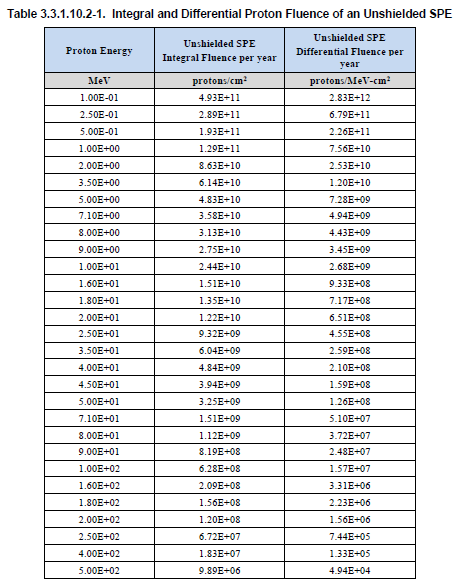
\includegraphics[scale=1.0]{DSNE_3.3.1.10.2-1.png}
	\caption{The unshielded SPE integral and differential fluence as defined in DSNE.}\label{fig:DSNE_UnshieldedSPEFlux}
\end{figure}

The SPE integral flux can be fit using a Weibull function, given by
\begin{equation}
\Phi(>E[MeV]) [\# cm^{-2}] = 9.278\times 10^{11} \exp\left(-1.821E^{0.298}\right),
\end{equation}
or by a double power law,
\begin{equation}
\Phi(>E[MeV]) [\# cm^{-2}] = \frac{1.248\times 10^{11}}{\left(\frac{E}{13.5}\right)^{2.587} + E^{0.6244}}.
\end{equation}

Shorter time periods than 1 year should not be scaled linearly. Most of the SPE flux is dominated by a few large SPEs, each occurring over at most 1 week.

Other SPE definitions may also be generated directly from the October 1989 SPE, especially for single event effects (SEE). Rates attributed to the peak 5-minute, worst day, and worst week fluxes are often used to define the SPE SEE environment for interplanetary space. Since this analysis is only concerned about TID, a more statistical approach is used, i.e., the ESP/PSYCHIC models.

%%%%%%%%%%%%%%%%%%%%%%%%%%%%%%%%%%%%%%%%%%%%%%%%%%%%%%%%%%%%%%%%%%
%%%%%%%%%%%%%%%%%%%%%%%%%%%%%%%%%%%%%%%%%%%%%%%%%%%%%%%%%%%%%%%%%%
\section{Dose Estimation}

Given the limited information available, the total ionizing dose (TID) is estimated in composites. The zeroth order estimation uses the DSNE SPE TID tables, which must assume a finite shielding thickness, shown in Section \ref{ssec:DSNEwithShielding}. A first order approximation is done by computing dose-depth curves in composites for various energies and incident angles, shown in Section \ref{ssec:SRIMnoShielding}.

Interestingly, using the DSNE tables, the conservative dose estimate assuming at least 3 mils of aluminum shielding is $7.59E4$ rads (which $3$ mils of shielding is outside the validity range of SHIELDOSE2, and the dose is in silicon), whereas the dose estimate using SRIM with no shielding in a carbon composite is $6.94E4$ rads. Half of the TID is deposited in the first $\sim15$ mils of composite material.

Using Figure \ref{fig:Dose_vs_IonEnergy} it can be concluded that the $3$ mils of aluminum shielding absorbed at least $20\%$ of the TID available. This would put the upper-end dose estimate using DNSE with shielding removed to be roughly $9.5E4$ rads.

%%%%%%%%%%%%%%%%%%%%%%%%%%%%%%%%%%%%%%%%%%%%%%%%%%%%%%%%%%%%%%%%%%
%%%%%%%%%%%%%%%%%%%%%%%%%%%%%%%%%%%%%%%%%%%%%%%%%%%%%%%%%%%%%%%%%%
\subsection{DSNE with Shielding}\label{ssec:DSNEwithShielding}

To use the DSNE to estimate dose in composites, a finite shielding layer is forced on the analysis\footnote{The DSNE TID tables in concern were developed using SHEILDOSE2, which implicitly assumes a finite range of shielding thicknesses.}. TID produced by DSNE Table 3.3.1.10.2-1 (Figure \ref{fig:DSNE_UnshieldedSPEFlux}) can be found in DSNE Table 3.3.1.10.2-3, also shown here in Figure \ref{fig:DSNE_UnshieldedSPETID}.

\begin{figure}[h!]
	\centering
	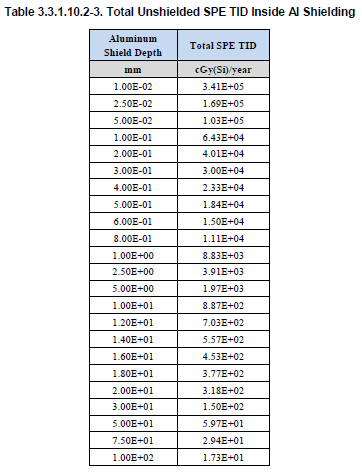
\includegraphics[scale=1.0]{DSNE_3.3.1.10.2-3.png}
	\caption{The TID in silicon as a function of aluminum shielding from unshielded SPE fluence as defined in DSNE.}\label{fig:DSNE_UnshieldedSPETID}
\end{figure}

The principle idea to compute dose in a composite using DSNE is to first compute the dose with only a thin amount of shielding. In this analysis, two thicknesses of MLI have been considered ($11.1$ and $3.05$ mils of aluminum equivalent thickness), shown in Table \ref{tab:al_equiv_MLI}. Dose in silicon after this MLI shielding is denoted by $D_{\text{MLI}}$. The next step is to add the thickness of the MLI layer and the composite layer (Table \ref{tab:thickness_comp}, spanning 31.5 to 748 mils of composite) as a single layer of aluminum equivalent thickness and compute the dose, $D_{\text{MLI+Composite}}$. The dose in only the composite is then computed by the difference between these two doses,
\begin{equation}
D_{\text{composite}} = D_{\text{MLI}} - D_{\text{MLI+Composite}}.
\end{equation}

To compute a dose $D_{\text{layer}}$ from DSNE Table 3.3.1.10.2-3 (Figure \ref{fig:DSNE_UnshieldedSPETID}), a power law interpolation scheme can be used to estimate dose for a shielding thickness $x_{\text{layer}}$ between two rows in the table. The interpolation scheme for the layer dose is given by
\begin{equation}
D_{\text{layer}} = D_i\left(\frac{D_{i+1}}{D_i}\right)^{\frac{\log(x_{\text{layer}}/x_i)}{\log(x_{i+1}/x_i})},
\end{equation}
where $x_{i+1} \ge x_{\text{layer}} > x_i$, for $x$ in units of mm and $D$ in units of cGy(Si) per year.

\begin{table}[h]\centering
	\caption{Estimation of dose using DSNE Table 3.3.1.10.2-3 in composites with two MLI shielding thicknesses and three composites each with two thicknesses (31.5 mils and 748 mils of composite). Thicknesses of MLI and composites were converted to aluminum equivalent thicknesses. The correction factor for each composite (Table \ref{tab:correction_factors}) is used to derive the aluminum equivalent thickness.}\label{tab:dose_composite_DSNE}
	\begin{tabular}{|c | c | c |}\hline
			 &Thin MLI (3.05 mils Al) & Thick MLI (11.1 mils Al) \\\hline
		Composite & TID dose [rad] &  TID dose [rad] \\\hline
		Thin glass (23.3 mils Al)   & 6.312E4 & 2.123E4 \\\hline
		Thick glass (554 mils Al)   & 7.594E4 & 3.083E4 \\\hline
		Thin aramid (20.3 mils Al)  & 6.130E4 & 2.023E4\\\hline
		Thick aramid (482 mils Al)  & 7.581E4 & 3.070E4\\\hline
		Thin carbon (22.1 mils Al)  & 6.246E4 & 2.086E4\\\hline
		Thick carbon (526 mils Al) & 7.589E4 & 3.078E4\\\hline
	\end{tabular}
\end{table}

Examining Table \ref{tab:dose_composite_DSNE}, the range of doses is from $2.023E4$ rad to $7.594E4$ rad. Any finite amount of shielding can limit the dose to the composite layer. The doses estimated using the thin MLI case are just above the minimum limit of $0.05$ mm (or $2$ mils) that SHIELDOSE2 can handle\footnote{\url{https://www.spenvis.oma.be/help/background/shieldose/shieldose.html}}\textsuperscript{,}\footnote{\url{https://www.spenvis.oma.be/help/models/sd2q.html}}. It is expected that by removing the MLI shielding, the estimated doses will be greater (by at least $25\%$) than the $7.594E4$ rad upper limit shown in Table~\ref{tab:dose_composite_DSNE}. However, further analysis is required to sharpen this dose estimate in composites. In Section \ref{ssec:SRIMnoShielding}, dose estimates in higher fidelity composite surrogates using SRIM with no shielding is discussed.


%%%%%%%%%%%%%%%%%%%%%%%%%%%%%%%%%%%%%%%%%%%%%%%%%%%%%%%%%%%%%%%%%%
%%%%%%%%%%%%%%%%%%%%%%%%%%%%%%%%%%%%%%%%%%%%%%%%%%%%%%%%%%%%%%%%%%
\subsection{SRIM without Shielding}\label{ssec:SRIMnoShielding}

The Stopping and Range of Ions in Matter (SRIM) \citep{ziegler2009srim} is a group of programs that calculate the stopping and range of ions in matter\footnote{\url{http://www.srim.org/SRIM/SRIMINTRO.htm}}. The ion stopping and range table calculator in SRIM was used in Section \ref{sssec:ProtonStoppingDistance}. For each run using TRIM (Transport of Ions in Matter), a mono-energetic beam of a single incident angle is used at the environment and transported through a series of predefined layers in a Monte Carlo fashion.

The isotropic flux for a particular energy and incident angle $\Phi(E,\theta)$ can be computed as (using a cosine distribution for an incident isotropic distribution on a flat slab)
\begin{equation}
\Phi(E,\theta) = [\Phi(E_i) - \Phi(E_{i+1})] \frac{\cos(2\theta_i) - \cos(2\theta_{i+1})}{2},
\end{equation}
where $E = \sqrt{E_i E_{i+1}}$, $\theta = (\theta_i + \theta_{i+1})/2$, and $\Phi(E_i)$ is the integral flux at energy $E_i$ (e.g., DSNE Table 3.3.1.10.2-1, or Figure \ref{fig:DSNE_UnshieldedSPEFlux}). The TRIM simulation is ran using $E$ and $\theta$ as centered values in the energy-angle bin. The anglular weight term follows from the integral
\begin{equation}
w_i = 2\int_{\theta_i}^{\theta_{i+1}}d\theta\sin\theta\cos\theta = \frac{\cos(2\theta_i) - \cos(2\theta_{i+1})}{2},
\end{equation}
were it is assumed that the incident angle $\theta$ ranges\footnote{Initially, the range of the incident angle is from $-90^\circ$ to $90^\circ$, but it is assumed the dose profiles will be symmetric about $0^\circ$.} from $0^\circ$ to $90^\circ$, hence the factor of $2$. In this analysis, the range of incident angles $\theta$ are given in Table \ref{tab:incidentAngleBins}.

\begin{table}[h]\centering
	\caption{Angular weight factors $w_i$ where $\sum_i w_i = 1$. The $\theta_i$ and $\theta_{i+1}$ are bin edges where $\theta$ is taken as the approximate bin center.}\label{tab:incidentAngleBins}
	\begin{tabular}{|c | c | c | c | c |}\hline
		index $i$ & $\theta_i$ & $\theta_{i+1}$ & $\theta$ & $w_i$ \\\hline
		0  & 0.00 & 15.0 & 0.00 & 3.40E-2 \\\hline
		1  & 15.0 & 37.5 & 30.0 & 1.73E-1 \\\hline
		2  & 37.5 & 52.5 & 45.0 & 1.85E-1\\\hline
		3  & 52.5 & 67.5 & 60.0 & 2.26E-1 \\\hline
		4  & 67.5 & 82.5 & 75.0 & 2.52E-1\\\hline
    	5  & 82.5 & 90.0 & 87.0 & 1.30E-1\\\hline
	\end{tabular}
\end{table}

TID can be computed by saving the ionization file once a sufficient number of test particles are ran. The ionization file contains information about the deposited ionization energy due to the primary ions $D_{\text{ions}}$ and to secondaries $D_{\text{recoils}}$ (called recoils) as a function of target depth. The ionization energy units are in eV per Angstrom per ion. To convert the deposited energy into rads, as a function of incident ion energy, angle and deposited depth, the following conversion equation is used
\begin{equation}
D(E,\theta,r) = [D_{\text{ions}} + D_{\text{recoils}}](r) \times \frac{10^8 \text{ \si{\angstrom}}}{\text{cm}} \times \frac{1.60218\times 10^{-19} \text{ J}}{\text{eV}} \times \frac{\Phi(E,\theta)}{\rho[\text{kg cm$^{-3}$}]} ,
\end{equation}
where $\rho$ is the material density in units of kg cm$^{-3}$. The dose as a function of energy or as a function of depth (see Figure \ref{fig:LayerDoseinSlab_vs_Depth}) can be calculated by summing over the other variables.

\begin{figure}[h!]
	\centering
	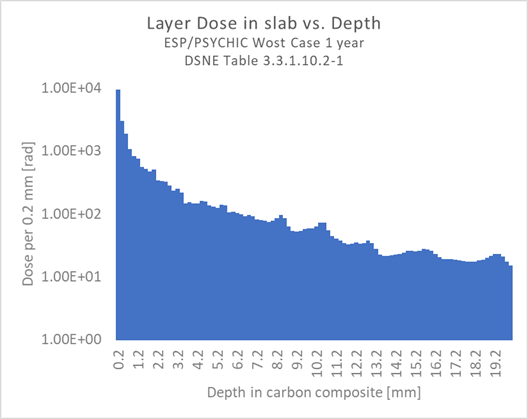
\includegraphics[scale=0.9]{LayerDoseinSlab_vs_Depth.png}
	\caption{Dose per 0.2 mm as a function of depth in a slab using DSNE Table 3.3.1.10.2-1 as the ion environment.}\label{fig:LayerDoseinSlab_vs_Depth}
\end{figure}

The dose-depth profile in a carbon composite is shown in Figure \ref{fig:LayerDoseinSlab_vs_Depth} for a composite thickness of $20$ mm. Artifacts can be seen at larger depth since a finite number of energies were probed. The spikes are due to individual Bragg peaks. With a greater number of energies probed, these spikes would be smoothed out.

Another way to look at the dose profile is total dose as a function of thickness, shown in Figure \ref{fig:TotalDoseinSlab_vs_Thickness}.

\begin{figure}[h!]
	\centering
	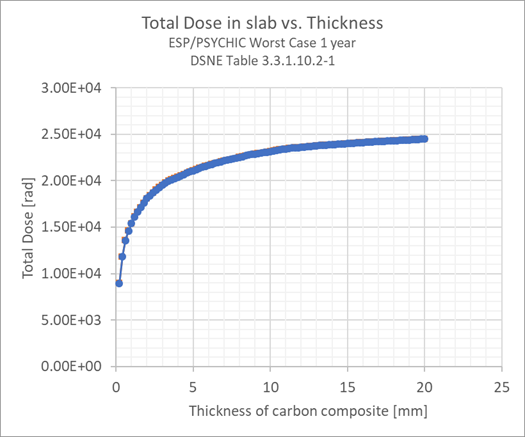
\includegraphics[scale=0.9]{TotalDoseinSlab_vs_Thickness.png}
	\caption{Total dose as a function of carbon composite thickness in a slab using DSNE Table 3.3.1.10.2-1 as the ion environment.}\label{fig:TotalDoseinSlab_vs_Thickness}
\end{figure}

The dose as a function of ion energy is given in Figure \ref{fig:Dose_vs_IonEnergy}, which is independent of geometry type, slab or sphere. In Section \ref{ssec:DSNEwithShielding}, the thinnest shielding assumed was $7.76\times 10^{-2}$ mm of aluminum equivalent. Using Table \ref{tab:stopping_distance}, energies less than $2.8$ MeV would be completely absorbed in the aluminum shielding. Therefore, using Figure \ref{fig:Dose_vs_IonEnergy} it can be concluded that the thin shielding absorbed at least $20\%$ of the TID available. This would put the upper-end dose estimate using DNSE to be roughly $9.5E4$ rads.

\begin{figure}[h!]
	\centering
	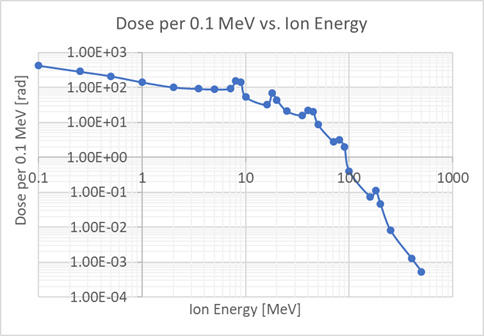
\includegraphics[scale=0.9]{Dose_vs_IonEnergy.png}
	\caption{Dose per 0.1 MeV as a function of ion energy using DSNE Table 3.3.1.10.2-1 as the ion environment.}\label{fig:Dose_vs_IonEnergy}
\end{figure}

In order to compare total doses computed in SRIM with the DSNE dose estimates done in Section \ref{ssec:DSNEwithShielding}, the slab doses must be converted to doses in a sphere. Equation~(9) of \cite{seltzer1986conversion} enables the determination of doses in a sphere, which is given by
\begin{equation}\label{eq:seltzer86_Eq9}
D_{\text{sphere}}(0,r) = 2\left[D_{\text{slab}}(r) - r\frac{d D_{\text{slab}}(r)}{dr}\right].
\end{equation}
To better approximate the derivative term, a power law interpolation fit can be made between each dose-depth pair. The dose in a slab can be approximated as
\begin{equation}\label{eq:slab_dose_power_law}
D_{\text{slab}}(r) \approx D_i\left(\frac{D_{i+1}}{D_i}\right)^{\frac{\log(r/r_i)}{\log(r_{i+1}/r_i)}},
\end{equation}
where $r_{i+1} \ge r \ge r_i$ and the $D_i$'s are the doses at depth $r_i$. Taking the derivative of Equation \eqref{eq:slab_dose_power_law},
\begin{equation}
\frac{d D_{\text{slab}}(r)}{dr} = \frac{\log\left(\frac{D_{i+1}}{D_i}\right)}{\log\left(\frac{r_{i+1}}{r_i}\right)}\frac{D_{\text{slab}}(r)}{r},
\end{equation}
and plugging into Equation \eqref{eq:seltzer86_Eq9}, the dose at the center of a sphere of radius $r$ now reads
\begin{equation}\label{eq:seltzer86_Eq9-powerlawDose}
D_{\text{sphere}}(0,r) \approx 2 D_{\text{slab}}(r)\left[1 - \frac{\log\left(\frac{D_{i+1}}{D_i}\right)}{\log\left(\frac{r_{i+1}}{r_i}\right)}\right].
\end{equation}
To better approximate the derivative term (which is used in this analysis), $r$ can be taken to be $r_{i+1}$ and use both the left and right sided approximation (this works if $i\ne 0$ or $i+1\ne N-1$, where $N$ is the total number of depths) so that the dose in a sphere can be written as
\begin{equation}\label{eq:seltzer86_Eq9-powerlawDose2}
D_{\text{sphere}}(0,r_{i+1}) \approx 2 D_{\text{slab}}(r_{i+1})\left[1 - \frac{\log\left(\frac{D_{i+1}}{D_i}\right)/\log\left(\frac{r_{i+1}}{r_i}\right) + \log\left(\frac{D_{i+2}}{D_{i+1}}\right)/\log\left(\frac{r_{i+2}}{r_{i+1}}\right)}{2}\right].
\end{equation}

After resampling the depth bins to a lower resolution to avoid the artifact jumps (which would mess up the derivative term), Figures \ref{fig:LayerDoseinSlab_vs_Depth} and \ref{fig:TotalDoseinSlab_vs_Thickness} are converted to doses in a sphere, shown in Figures \ref{fig:LayerDoseinSphere_vs_Depth} and \ref{fig:TotalDoseinSphere_vs_Thickness}, respectively.

\begin{figure}[h!]
	\centering
	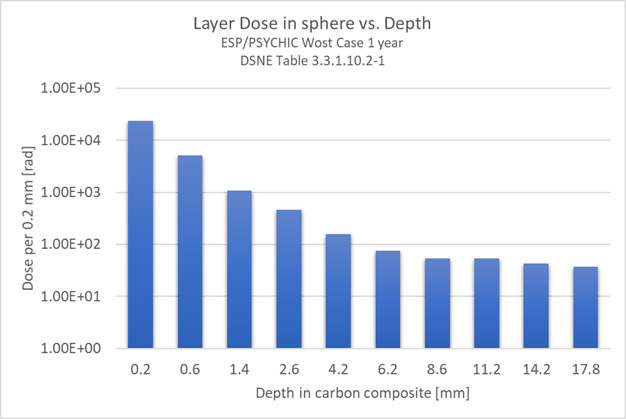
\includegraphics[scale=0.9]{LayerDoseinSphere_vs_Depth.png}
	\caption{Dose per 0.2 mm as a function of depth in a sphere using DSNE Table 3.3.1.10.2-1 as the ion environment.}\label{fig:LayerDoseinSphere_vs_Depth}
\end{figure}

\begin{figure}[h!]
	\centering
	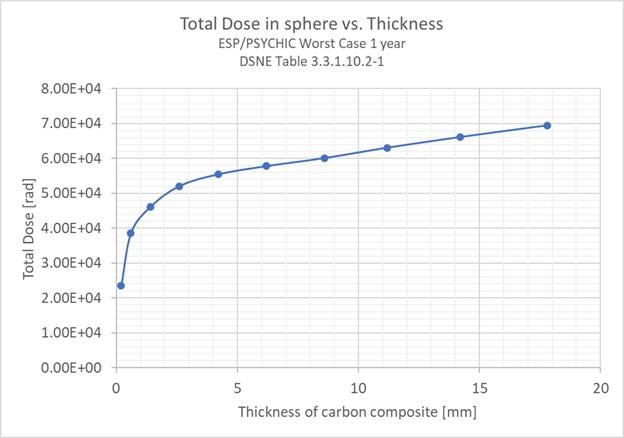
\includegraphics[scale=0.9]{TotalDoseinSphere_vs_Thickness.png}
	\caption{Total dose as a function of carbon composite thickness in a sphere using DSNE Table 3.3.1.10.2-1 as the ion environment.}\label{fig:TotalDoseinSphere_vs_Thickness}
\end{figure}

From Figure \ref{fig:TotalDoseinSphere_vs_Thickness}, the TID absorbed by $20$ mm of carbon composite is $6.94\times 10^{4}$~rads. Half of this total dose is absorbed in the first $0.4$ mm or $15$ mils of the carbon composite, and $75\%$ of the total dose is absorbed in the first $2.5$ mm or $100$ mils of carbon composite.


%%%%%%%%%%%%%%%%%%%%%%%%%%%%%%%%%%%%%%%%%%%%%%%%%%%%%%%%%%%%%%%%%%
%%%%%%%%%%%%%%%%%%%%%%%%%%%%%%%%%%%%%%%%%%%%%%%%%%%%%%%%%%%%%%%%%%
\section{SRIM Comparison with DSNE (SHIELDOSE2)}

The doses computed in SRIM are compared with DSNE Table 3.3.1.10.2-3 (see Figure \ref{fig:DSNE_UnshieldedSPETID}). First, the SRIM doses are computed in a slab using the SPE worst case 1 year environment (DSNE Table 3.3.1.10.2-1) and are compared with doses computed in SPENVIS. The same exact set of knobs is used in computing DSNE Table~3.3.1.10.2-3, except the \textsf{slab} option is used instead. It doesn't matter whether a finite or infinite slab is used. Both were checked and there were no differences with this particular energy spectrum and ion (protons). The SRIM doses in a slab and sphere are summarized in Table \ref{tab:SRIM_doses} and comparisons with SHIELDOSE2 (see Appendix \ref{asec:SPENVISOutput}) are shown in Figure \ref{fig:Dose_vs_shielding_slab_comparison}.

\begin{table}[h]\centering
	\caption{Dose to silicon in slab and spherical geometric as a function of aluminum shielding thickness. Equation \eqref{eq:seltzer86_Eq9-powerlawDose2} was used to convert slab doses to sphere doses.}\label{tab:SRIM_doses}
	\begin{tabular}{|c | c | c |}\hline
		Al thickness [mm] & Dose in slab [rad] & Dose in sphere [rad]  \\\hline
		1.0E-2 & 1.57E5 & 5.45E5 \\\hline
		1.0E-1 & 3.31E4 & 1.15E5 \\\hline
		1.0E+0 & 3.52E3 & 1.29E4 \\\hline
		1.0E+1 & 2.73E2 & 1.07E3 \\\hline
		1.0E+2 & 4.54E0 & 2.63E1 \\\hline
	\end{tabular}
\end{table}

\begin{figure}[h!]
	\centering
	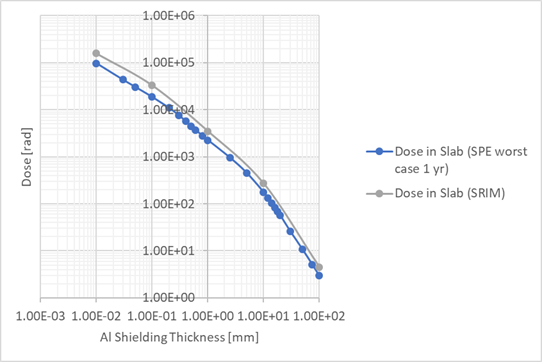
\includegraphics[scale=0.9]{Dose_vs_shielding_slab_comparison.png}
	\caption{Comparison between slab dose as a function of aluminum shielding thickness of SRIM and SPENVIS (i.e., SHIELDOSE2) runs.}\label{fig:Dose_vs_shielding_slab_comparison}
\end{figure}

The doses computed in SRIM are consistently overestimated compared with SHIELDOSE2, which is a consequence of low-resolution sampling of the energy-angle space of the incident ion spectrum. In this analysis, only normally incident ions were considered. One calculation was done with a shielding thickness of $1$ mm that took into account additional angular information of the isotropic spectrum. The estimated dose in silicon of spherical geometry turned out to be $8.55\times 10^{3}$ rads whereas the DSNE value is $8.83\times 10^{3}$ rads. This shows that better angular resolution could lower the SRIM dose estimates shown in Figure \ref{fig:Dose_vs_shielding_slab_comparison}.

\begin{figure}[h!]
	\centering
	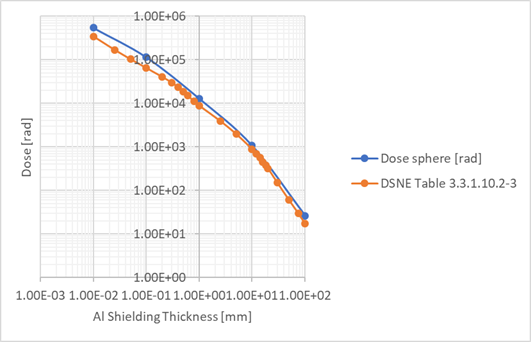
\includegraphics[scale=0.9]{Dose_vs_shielding_sphere_comparison.png}
	\caption{Comparison between sphere dose as a function of aluminum shielding thickness of SRIM and SPENVIS (i.e., SHIELDOSE2) runs.}\label{fig:Dose_vs_shielding_sphere_comparison}
\end{figure}

The SRIM-DSNE comparison shown in Figure \ref{fig:Dose_vs_shielding_sphere_comparison} is in much better agreement, which is a way of validation of SRIM for the analysis given in Section \ref{ssec:SRIMnoShielding}.

%%%%%%%%%%%%%%%%%%%%%%%%%%%%%%%%%%%%%%%%%%%%%%%%%%%%%%%%%%%%%%%%%%
%%%%%%%%%%%%%%%%%%%%%%%%%%%%%%%%%%%%%%%%%%%%%%%%%%%%%%%%%%%%%%%%%%

\appendix
\addcontentsline{toc}{section}{Appendix}
\section{Ion Stopping and Range Tables}
\label{asec:IonStoppingRangeTables}

\lstinputlisting[language=XML,basicstyle=\footnotesize,frame=single,
caption={Ion stopping and range tables of protons in glass composite.},label=lst:glass_composite]{Hydrogen in Glass Composite.txt}

\lstinputlisting[language=XML,basicstyle=\footnotesize,frame=single,
caption={Ion stopping and range tables of protons in aramid composite.},label=lst:aramid_composite]{Hydrogen in Aramid Composite.txt}

\lstinputlisting[language=XML,basicstyle=\footnotesize,frame=single,
caption={Ion stopping and range tables of protons in carbon composite.},label=lst:carbon_composite]{Hydrogen in Carbon Composite.txt}

\lstinputlisting[language=XML,basicstyle=\footnotesize,frame=single,
caption={Ion stopping and range tables of protons in aluminum.},label=lst:aluminum]{Hydrogen in Aluminum.txt}


\section{SPENVIS Output}
\label{asec:SPENVISOutput}

\lstinputlisting[language=XML,basicstyle=\footnotesize,frame=single,
caption={ESP PSYCHIC SPE worst case 1 year.},label=lst:SPEworstcase]{../ESP-PSYCHIC_SPE-worst_case_1yr.txt}

\lstinputlisting[language=XML,basicstyle=\footnotesize,frame=single,
caption={Dose in silicon as a function of aluminum shielding thickness of a sphere.},label=lst:DoseSphere]{../Dose_SPE-worst_case_1yr-sphere.txt}

\lstinputlisting[language=XML,basicstyle=\footnotesize,frame=single,
caption={Dose in silicon as a function of aluminum shielding thickness of a slab.},label=lst:DoseSlab]{../Dose_SPE-worst_case_1yr-slab.txt}


%\section{References}
\cleardoublepage
\phantomsection
\addcontentsline{toc}{section}{References}
\bibliographystyle{agu}
\bibliography{report}

\end{document}